\documentclass[11pt]{article}
\usepackage[margin=1.0in]{geometry}
\addtolength{\topmargin}{0.25in}
\usepackage[document]{ragged2e}
\usepackage{graphicx}
\graphicspath{ {../pictures/} }
\usepackage{float}
\usepackage{siunitx}


\begin{document}
	{\Huge\textbf{EEE381 Tech Memo}}\\
	\hfill \break
	\textbf{From:} Charles Noah Lutz\\
	\textbf{Partner:} N/A\\
	\textbf{To:} Colin Bussert\\
	\textbf{Date:} Performed: 09/20/18; Due: 09/27/18\\
	\textbf{Subject:} Lab \#01

	\section{Abstract}
	The goal of this exercise was to observe the relationship between the
	voltage and current through a diode and extract the leakage current, \(I_{s}\), and
	the diode non-ideality factor, \(n\). In addition, a half-wave rectifier was simulated
	and built in order to evaluate its performance.

	\section{Theory}
	\label{sec:theory}
	In order to find the leakage current \(I_{s}\) and the diode non-ideality factor \(n\),
	the diode current and voltage relationship must be understood. The expression for 
	current through a diode can be seen in Equation \ref{equ:i_diode}.

	\begin{equation}
		\label{equ:i_diode}
		i_{D} = I_{s} (\exp(qV_{D}/nkT)-1)
	\end{equation}

	Assuming that \(V_{D} >> 0\), this equation can be simplified slightly to the form
	seen in Equation \ref{equ:i_diode_simple}.
	\begin{equation}
		\label{equ:i_diode_simple}
		i_{D} = I_{s} \exp(qV_{D}/nkT)
	\end{equation}
	
	When the natural log of \(i_{D}\) is plotted against \(V_{D}\), the slope of the
	resulting line is a function of \(n\) (Equation \ref{equ:lni_diode}).
	\begin{equation}
		\label{equ:lni_diode}
		\ln(i_{D}) = \ln(I_{s}) + (\frac{q}{nkT})V_{D}
	\end{equation}

	Assuming room tempurature, the value of \(n\) can be found by looking at the slope
	of the line of Equation \ref{equ:lni_diode}.\\
	\hfill \break
	The value of \(I_{s}\) can be found by looking at the current when the y-intercept,
	which is equal to the natural log of \(I_s\). This value is usually very small 
	(in the nano/pico Amp range).\\
	\hfill \break
	A PSpice circuit was created to model this behavior and can be seen in Figure 
	\ref{fig:diode1}.

	\begin{figure}[H]
		\centering
		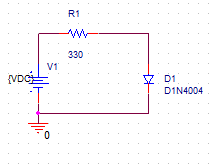
\includegraphics{diode_circuit.png}
		\caption{Basic diode circuit used for \(I_s\) and \(n\) parameter extraction}
		\label{fig:diode1}
	\end{figure}

	A DC Sweep simulation was run to find the \(i_D-V_D\) relationship and then extract
	the \(I_s\) and \(n\) values. The graph of the \(i_D-V_D\) curve can be seen in 
	Figure \ref{fig:id_vd_curve}.

	\begin{figure}[H]
		\centering
		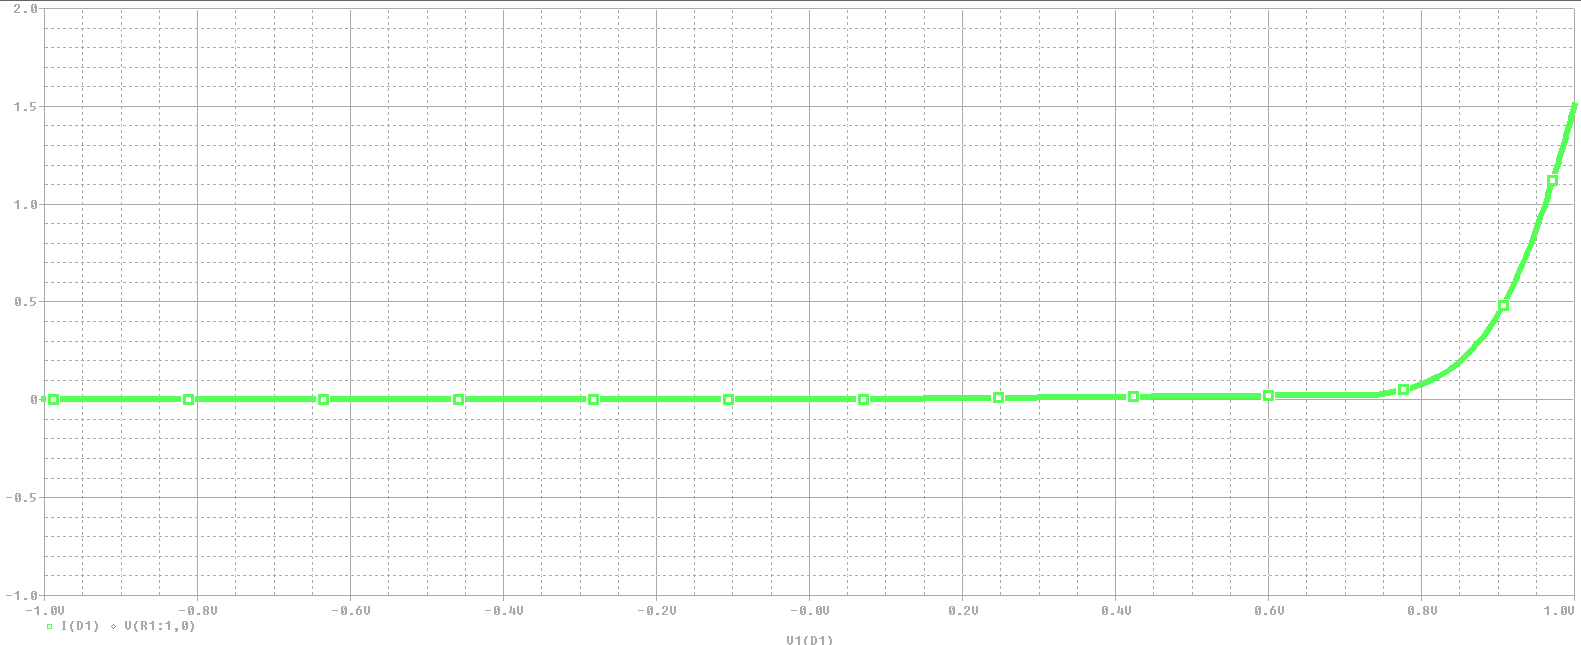
\includegraphics[width=\textwidth]{Id-Vd_DC_Sweep.png}
		\caption{\(i_D\) vs. \(V_D\) graph}
		\label{fig:id_vd_curve}
	\end{figure}

	Using this graph, the \(I_s\) parameter can be extracted. For the 1N4004 diode, the 
	\(I_s\) value was found to be roughly 500 \si{\pico\ampere}. For the extraction of
	the \(n\) parameter, \(i_d\) needs to be graphed on a logarithmic scale, then the slope
	of the resulting line gives the \(n\) value. The value that was found during simulation
	based of the graph in Figure \ref{fig:id_vd_curve} was \(n = 1.4815\).\\

	\hfill\break

	The second circuit that was simulated was the half-wave rectifier circuit that is shown
	in Figure \ref{fig:half-wave_rectifier}.

	\begin{figure}[H]
		\centering
		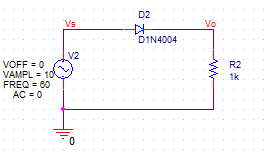
\includegraphics{half_wave_rectifier.png}
		\caption{Half-wave rectifier circuit with 1\si{\kilo\ohm} load}
		\label{fig:half-wave_rectifier}
	\end{figure}

	The purpose of this circuit is to change the sinusoidal (AC) source to 
	something closer to a DC source. The diode blocks current flowing backwards, 
	causing the voltage across the resistor to never go negative and have a positive
	average value. In this case, the AC source has a peak voltage of 10 \si{\volt} and
	a frequency of 60 \si{\hertz}. If the diode in Figure \ref{fig:half-wave_rectifier}
	were ideal, then the voltage across the resistor would follow the positive voltages 
	from the source exactly and be zero when the source voltage went negative. Because
	it is a non-ideal diode, the voltage across the resistor does not follow the source 
	voltage exactly. It can be modeled ,using the constant voltage drop model, as
	a voltage source and a resistor in series. The value of the voltage source is always 
	assumed to be 0.7 \si{\volt} and the value of the resistor can be derived by looking 
	at the voltage across the resistor vs. the voltage from the source. This graph can 
	be seen in Figure \ref{fig:half-wave_rectifier_graph}.

	\begin{figure}[H]
		\centering
		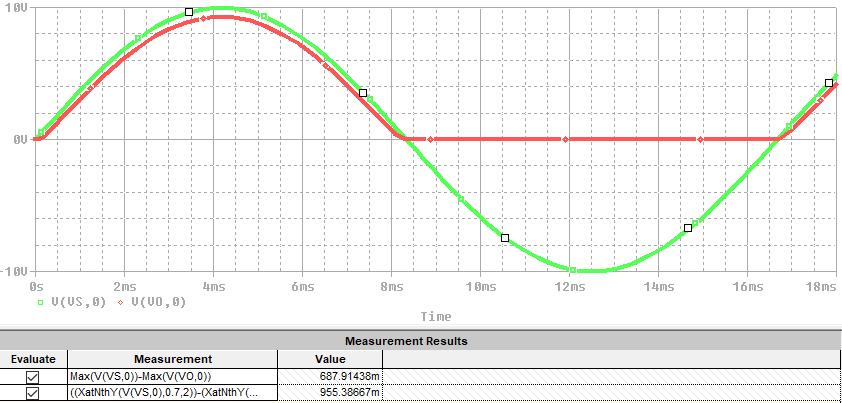
\includegraphics[width=\textwidth]{half_wave_rectifier_graph.png}
		\caption{Half-wave rectifier input vs. output}
		\label{fig:half-wave_rectifier_graph}
	\end{figure}

	Another value that is important to look at when using rectifiers is the conductance
	ratio, or the amount of time that diode is conducting, relative to the period of the
	signal that is being rectified. Ideally, this value would be exactly half the period 
	as the diode would conduct exactly when the source voltage goes positive. However,
	there is a short period of time where the diode is not conducting, despite the input
	voltage being positive. This is due to the fact that the voltage across the diod has
	to be roughly 0.7 \si\volt before the diode starts conducting. In Figure 
	\ref{fig:half-wave_rectifier_graph} the conduction ratio was found to be \(0.47769\).\\
	
	\hfill \break

	The final circuit that was simulated was another half-wave rectifier, but with a
	10 \si{\micro\farad} capacitor in parallel with the load resistor. This causes an 
	RC discharge circuit to form when the source voltage falls below zero and the diode
	stops conducting. This means that as long as the RC time constant is big enough 
	so that the capacitor does not discharge fully, the output signal looks much 
	more like a DC signal. This can be seen in Figure 
	\ref{fig:half-wave_rectifier_cap_graph}.

	\begin{figure}[H]
		\centering
		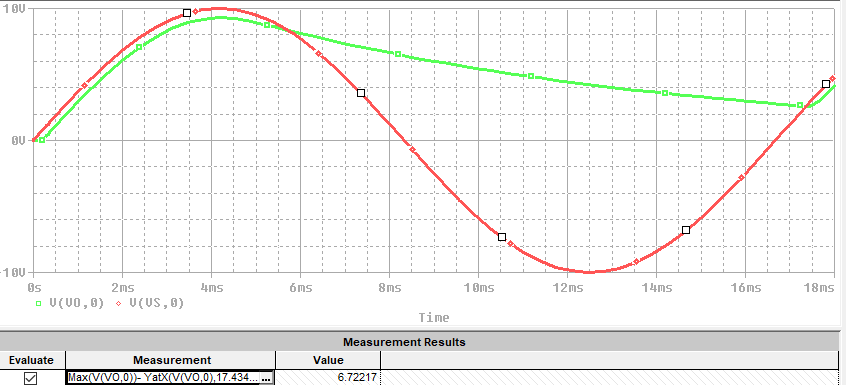
\includegraphics[width=\textwidth]{half_wave_rectifier_cap_graph.png}
		\caption{Half-wave rectifier input vs. output with parallel capacitor}
		\label{fig:half-wave_rectifier_cap_graph}
	\end{figure}

	The differnce between the peak output voltage and the voltage that the RC circuit
	drops to is called the ripple voltage (\(V_r\)). The smaller this value is, the
	closer the output signal is to an actual DC value. In this case, the ripple 
	voltage that was found in simulation was \(6.72217\) \si\volt.

	\section{Results and Discussion}
	The first circuit that was tested experimental was the circuit in Figure
	\ref{fig:diode1}. It was tested by using a DC power supply and applying
	various voltages from 1 \si\volt to 10 \si\volt and measuring the voltage
	drop across the resistor and the current draw that the power supply 
	experienced. This data can be seen in Table \ref{table:id_vd} and 
	in Figure \ref{fig:id_vd_graph_exp}.

	\begin{table}[H]
		\centering
		\caption{\(I_D\) vs \(V_D\) data}
		\label{table:id_vd}
		\begin{tabular}{|l|l|l|}
			\hline
			\(V_s\)(V) & \(V_D\)(V) & \(I_D\)(A)\\
			\hline
			1 & 0.6032 & 0.001\\
			2 & 0.6560 & 0.003\\
			3 & 0.6787 & 0.006\\
			4 & 0.6934 & 0.009\\
			5 & 0.7040 & 0.012\\
			6 & 0.7121 & 0.016\\
			7 & 0.7176 & 0.019\\
			8 & 0.7225 & 0.022\\
			9 & 0.7275 & 0.025\\
			10 & 0.7305 & 0.028\\
			\hline
		\end{tabular}
	\end{table}

	\begin{figure}[H]
		\centering
		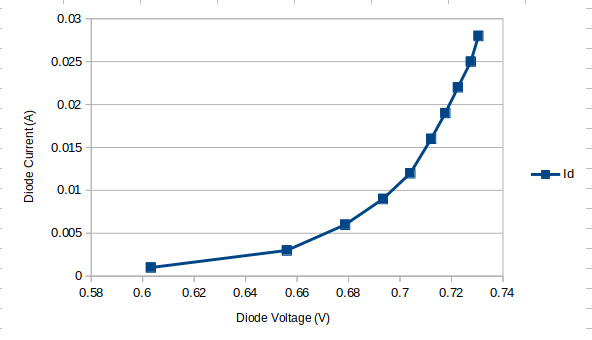
\includegraphics[width=\textwidth]{diode_Id_Vd_experimental.png}
		\caption{Graph of \(I_D\) vs \(V_D\) Experimental}
		\label{fig:id_vd_graph_exp}
	\end{figure}
	
	The extracted \(n\) value that was obtained from this data was 26.176. The 
	extracted value for \(I_s\) was -23.1906 \si\ampere. These values were extremley
	far off from the values found during simulation. This could have been due to 
	the fact that the measurements were incorrectly taken, the circuit was improperly
	set up, or the way the values were calculated was incorrect.\\
	
	\hfill \break

	The next circuit that was built in lab was the half-wave recitifier from 
	Figure \ref{fig:half-wave_rectifier}. The circuit was powered using a 
	waveform generator generating a 10\si{\volt} peak-peak sinusoidal signal with 
	a frequency of 60\si{\hertz}. (Note: this is the improper setup as the 
	signal should have been a 10\si{\volt} amplitude as it was in simulation,
	not peak-peak). The circuit was monitored using an oscilloscope and 
	the output can be seen in Figure \ref{fig:half-wave_rectifier_graph_exp}.

	\begin{figure}[H]
		\centering
		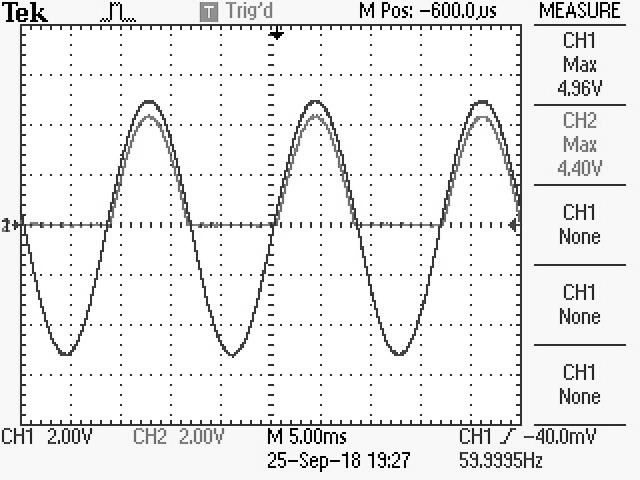
\includegraphics{half_wave_rectifier_graph_exp.JPG}
		\caption{Oscilloscope capture of half-wave rectifier in Figure \ref{fig:half-wave_rectifier}}
		\label{fig:half-wave_rectifier_graph_exp}
	\end{figure}

	Using the data captured by the oscilloscope, the experimental conduction
	ratio was found to be 0.4692. This value is relativley close with the
	value for conduction ratio during simulation, despite the fact that
	the voltage source was improperly configured. This, however, makes sense due to
	the fact that the 5\si\volt peak is still much greater than the threshold
	voltage of 0.7\si\volt. This means that the diode is still conducting for 
	roughly the same amount of time during the period. The difference between 
	these two values can be attributed to the slight difference in the 
	amount of time it took for the simulated voltage across the diode to raise
	above 0.7\si{\volt} and the slightly longer amount of time that the experimental
	voltage across the diode to raise above 0.7\si{\volt} as the sinusoid with a larger
	peak voltage will cross 0.7\si{\volt} faster than a sinusoid with a lower peak
	voltage.\\

	\hfill \break

	The final circuit that was tested experimentally was the half-wave 
	rectifier circuit with the 10\si{\micro\farad} capacitor in parallel
	with the load resistor. As established in section \ref{sec:theory},
	this should produce an output signal much closer to a DC signal due to
	the RC circuit that forms. This circuit was powered with the same
	10\si{\volt} peak-peak, 60\si{\hertz} signal that the previous circuit
	was powered with. (Note: this is still incorrect as the simulation used
	at 10\si{\volt} amplitude signal, not peak-peak). The oscilloscope capture
	can be seen in Figure \ref{fig:half-wave_rectifier_cap_graph_exp}.

	\begin{figure}[H]
		\centering
		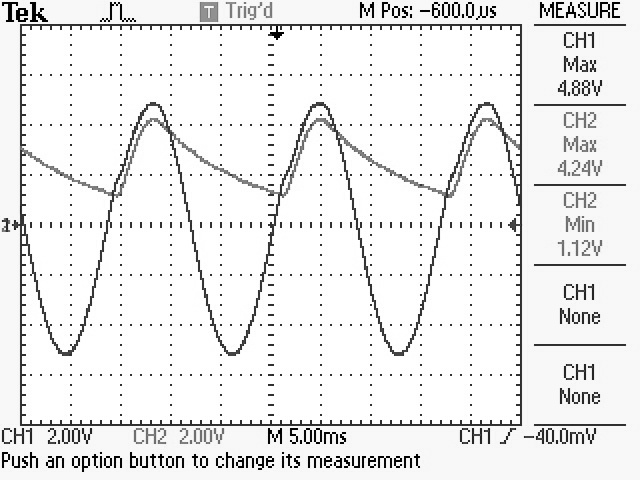
\includegraphics{half_wave_rectifier_cap_graph_exp.JPG}
		\caption{Half-wave rectifier with 10\si{\micro\farad} capacitor}
		\label{fig:half-wave_rectifier_cap_graph_exp}
	\end{figure}

	The experimentally found ripple voltage was 3.12\si{\volt}. While this
	is not close to the ripple voltage found during simulation, it can
	be attributed to the fact that the voltage source was improperly
	configured to be a 10\si{\volt} peak-peak signal. This means that the 
	voltage across the resistor and capacitor only rose to slightyly under 
	5\si{\volt}, rather than the 10\si{\volt} that it did in simulation,
	resulting in a significantly lower ripple voltage.\\

	\section{Conclusion}
	The goal for this exercise was to observe and extract properties
	of non-ideal diodes and to use diodes in a practical application. 
	The leakage current and non-ideality factors were extracted from 
	the diode \(I_D - V_D\) curve and the diodes were used in two 
	different half-wave rectifier circuits to convert an AC source
	into a more DC-like signal.\\
	
	\hfill \break

	Most experimental values matched the simulated values, other than 
	the leakage current and diode non-ideality factor. The others either
	matched almost exactly, or differences could be attributed to the fact
	that the voltage sources for the two half-wave rectifier circuits were
	improperly configured.
\end{document}
